\documentclass{article}
\usepackage[T1]{fontenc}
\usepackage{lmodern}
\usepackage{hyperref}
\usepackage[a4paper,left=10mm,right=10mm,top=15mm,bottom=15mm]{geometry}

\usepackage[french]{babel}

\usepackage{minted}
\usepackage{xcolor}
\usepackage{tcolorbox}
\usepackage{etoolbox}
\parindent=0pt
\usemintedstyle[mysql]{default}
\definecolor{bgcode}{rgb}{0.9,0.9,0.9}
\definecolor{bgconsole}{rgb}{0.0,0.0,0.0}
\usemintedstyle[console]{rrt}
\usepackage{xpatch}
\xpretocmd{\inputminted}{\begin{tcolorbox}}{}{}%
\xapptocmd{\inputminted}{\end{tcolorbox}}{}{}%

\BeforeBeginEnvironment{minted}{\begin{tcolorbox}}%
\AfterEndEnvironment{minted}{\end{tcolorbox}}%
\renewcommand{\listingscaption}[1][Code]{#1}
\renewcommand{\listoflistingscaption}{Liste des codes}

\title{Évaluation Intermédiaire - MySQL,base de donnée d’une librairie}
\author{Jean Lucien RANDRIANANTENAINA}

\begin{document}

\maketitle
\newpage
\tableofcontents
\newpage
\listoflistings
\newpage

\section{Analyse et correction de la base de données}

\subsection{Chargement de Biblio\_base.mysql}

\begin{listing}[H]
\inputminted{mysql}{code/create_db.sql}
\caption{Création de la base de donné  et changement de la base de donné courante}
\end{listing}

\begin{listing}[H]
\inputminted{mysql}{code/create_oeuvres.sql}
\caption{Création de la table oeuvres}
\end{listing}

\begin{listing}[H]
\inputminted{mysql}{code/create_adherents.sql}
\caption{Création de la table adherents}
\end{listing}

\begin{listing}[H]
\inputminted{mysql}{code/create_livres.sql}
\caption{Création de la table livres}
\end{listing}

\begin{listing}[H]
\inputminted{mysql}{code/create_emprunter.sql}
\caption{Création de la table emprunter}
\end{listing}

\begin{listing}[H]
\inputminted{mysql}{code/insert_oeuvres.sql}
\caption{Insertion de données dans la table oeuvres}
\end{listing}

\begin{listing}[H]
\inputminted{mysql}{code/insert_adherents.sql}
\caption{Insertion de données dans la table adherents}
\end{listing}

\newpage
\begin{listing}[H]
\inputminted{mysql}{code/insert_livres.sql}
\caption{Insertion de données dans la table livres}
\end{listing}

\newpage
\begin{listing}[H]
\inputminted{mysql}{code/insert_emprunter.sql}
\caption{Insertion de données dans la table emprunter}
\end{listing}

\subsection{Les corrections aporté}
    Ordonner l'ordre de la création des tables pour eviter les erreur
    suivant :
    
\begin{itemize}
    \item Error Code: 1824. Failed to open the referenced table `oeuvres'
    \item Error Code: 1824. Failed to open the referenced table `adherents'
    \item Error Code: 1824. Failed to open the referenced table `livres'
\end{itemize}


Ainsi l'ordre de création des tables sera :
\begin{enumerate}
    \item oeuvres
    \item adherants
    \item livres
    \item emprunter
\end{enumerate}

On a aussi deux ligné qui on des dates erroné dans la tables emprunter, dont la date de retour (\mintinline{mysql}{dateRet}) est antérieur  à la
date d'emprunt (\mintinline{mysql}{dateEmp})
\begin{listing}[H]
\begin{minted}{mysql}
    (26,from_days(to_days(current_date)-315),21,from_days(to_days(current_date)-318),9)
    (12,from_days(to_days(current_date)-300),21,from_days(to_days(current_date)-1290),7)
\end{minted}
\begin{minted}[bgcolor=bgconsole]{console}
                +----+------------+----------+------------+----+
                | NL | dateEmp    | dureeMax | dateRet    | NA |
                +----+------------+----------+------------+----+
                | 12 | 2021-08-31 |       21 | 2018-12-15 |  7 |
                | 26 | 2021-08-16 |       21 | 2021-08-13 |  9 |
                +----+------------+----------+------------+----+
                2 rows in set (0,00 sec)
\end{minted}
\caption{Erreur des enrégistrements dans la BD}
\end{listing}
Pour palier ce problème on ava mettre à jours ces deux enréstrement pour être cohérent avec les deux commandes suivantes :
\begin{center}
\begin{minipage}{0.5\linewidth}
\begin{listing}[H]
\begin{minted}{mysql}
UPDATE `biblio`.`emprunter` 
SET 
    `dateRet` = '2021-12-15'
WHERE
    (`NL` = '12')
        AND (`dateEmp` = '2021-08-31');
\end{minted}
\begin{minted}[bgcolor=bgconsole]{console}
Query OK, 1 row affected (0,13 sec)
Rows matched: 1  Changed: 1  Warnings: 0    
\end{minted}
\begin{minted}{mysql}
UPDATE `biblio`.`emprunter` 
SET 
    `dateRet` = '2021-08-19'
WHERE
    (`NL` = '26')
        AND (`dateEmp` = '2021-08-16');    
\end{minted}
\begin{minted}[bgcolor=bgconsole]{console}
    Query OK, 1 row affected (0,08 sec)
    Rows matched: 1  Changed: 1  Warnings: 0    
\end{minted}    
\caption{Correction des données}
\end{listing}
\end{minipage}
\end{center}
\subsection{Diagramme EER de biblio}
\begin{center}
    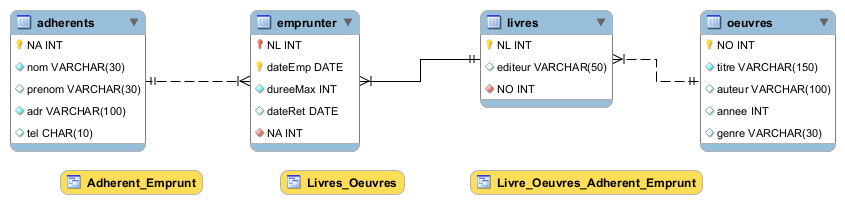
\includegraphics[scale=0.6]{EER_Diagram.png}
\end{center}

\subsection{Nombres de tuples après l'execution du script:}

\begin{center}
\begin{minipage}{0.45\linewidth}
Table oeuvres
\begin{listing}[H]
\begin{minted}{mysql}
SELECT COUNT(*) FROM `biblio`.`oeuvres`;
\end{minted}

\begin{minted}[bgcolor=bgconsole]{console}
+----------+
| COUNT(*) |
+----------+
|       18 |
+----------+
1 row in set (0,04 sec)
\end{minted}
	\caption{Nombre de tuples dans la table oeuvres}
\end{listing}
\end{minipage} \begin{minipage}{0.45\linewidth}
Table adherents :
\begin{listing}[H]
\begin{minted}{mysql}
SELECT COUNT(*) FROM `biblio`.`adherents`;
\end{minted}
\begin{minted}[bgcolor=bgconsole]{console}
+----------+
| COUNT(*) |
+----------+
|       30 |
+----------+
1 row in set (0,04 sec)
\end{minted}
\caption{Nombre de tuples dans la table adherants}
\end{listing}
\end{minipage}

\begin{minipage}{0.45\linewidth}
Table livres :
\begin{listing}[H]
\begin{minted}{mysql}
SELECT COUNT(*) FROM `biblio`.`livres`;
\end{minted}
\begin{minted}[bgcolor=bgconsole]{console}
+----------+
| COUNT(*) |
+----------+
|       32 |
+----------+
1 row in set (0,01 sec)
\end{minted}
\caption{Nombre de tuples dans la table livres}
\end{listing}
\end{minipage} \begin{minipage}{0.45\linewidth}
Table emprunter :
\begin{listing}[H]
\begin{minted}{mysql}
SELECT COUNT(*) FROM `biblio`.`emprunter`;
\end{minted}
\begin{minted}[bgcolor=bgconsole]{console}
+----------+
| COUNT(*) |
+----------+
|       33 |
+----------+
1 row in set (0,05 sec)	
\end{minted}
\caption{Nombre de tuples dans la table emprunter}
\end{listing}	
\end{minipage}

\textbf{Ainsi pour obtenir le nombre totale de Tuple on fait :}

\begin{minipage}{0.8\linewidth}
\begin{listing}[H]
\begin{minted}{mysql}
SELECT 
	(SELECT COUNT(*) FROM `biblio`.`oeuvres`) 
	+
	(SELECT COUNT(*) FROM `biblio`.`adherents`)
	+
	(SELECT COUNT(*) FROM `biblio`.`livres`)
	+
	(SELECT COUNT(*) FROM `biblio`.`emprunter`)
	AS `Nombres de tuples`;
\end{minted}
\begin{minted}[bgcolor=bgconsole]{console}
+-------------------+
| Nombres de tuples |
+-------------------+
|               113 |
+-------------------+
1 row in set (0,80 sec)
\end{minted}
\caption{Nombres de tuples (enregistrements) totale dans la base de donné}
\end{listing}	
\end{minipage}
\end{center}


\subsection{Nombre d'attribut dans chaque table}

Pour trouver le nombre d'attribut de chaque table on vas utiliser la commande \mintinline{mysql}{DESCRIBE}
\begin{center}
\begin{minipage}{0.8\linewidth}
Table oeuvres : 5 attributs
\begin{listing}[H]
\begin{minted}{mysql}
DESCRIBE `biblio`.`oeuvres`;
\end{minted}
\begin{minted}[bgcolor=bgconsole]{console}
+--------+--------------+------+-----+---------+----------------+
| Field  | Type         | Null | Key | Default | Extra          |
+--------+--------------+------+-----+---------+----------------+
| NO     | int          | NO   | PRI | NULL    | auto_increment |
| titre  | varchar(150) | NO   |     | NULL    |                |
| auteur | varchar(100) | YES  |     | NULL    |                |
| annee  | int          | YES  |     | NULL    |                |
| genre  | varchar(30)  | YES  |     | NULL    |                |
+--------+--------------+------+-----+---------+----------------+
5 rows in set (0,02 sec)
\end{minted}
\caption{Les 5 attributs de la tables oeuvre}
\end{listing}
\end{minipage}


\begin{minipage}{0.8\linewidth}
Table adherents : 5 attributs.
\begin{listing}[H]
\begin{minted}{mysql}
DESCRIBE `biblio`.`adherents`;
\end{minted}
\begin{minted}[bgcolor=bgconsole]{console}
+--------+--------------+------+-----+---------+----------------+
| Field  | Type         | Null | Key | Default | Extra          |
+--------+--------------+------+-----+---------+----------------+
| NA     | int          | NO   | PRI | NULL    | auto_increment |
| nom    | varchar(30)  | NO   |     | NULL    |                |
| prenom | varchar(30)  | YES  |     | NULL    |                |
| adr    | varchar(100) | NO   |     | NULL    |                |
| tel    | char(10)     | YES  |     | NULL    |                |
+--------+--------------+------+-----+---------+----------------+
5 rows in set (0,00 sec)
\end{minted}
\caption{Les 5 attributs de la table adhérents}
\end{listing}
\end{minipage}	

\vspace*{20pt}

\begin{minipage}{0.8\linewidth}
Table livres : 3 attributs
\begin{listing}[H]
\begin{minted}{mysql}
DESCRIBE `biblio`.`livres`;
\end{minted}
\begin{minted}[bgcolor=bgconsole]{console}
+---------+-------------+------+-----+---------+----------------+
| Field   | Type        | Null | Key | Default | Extra          |
+---------+-------------+------+-----+---------+----------------+
| NL      | int         | NO   | PRI | NULL    | auto_increment |
| editeur | varchar(50) | YES  |     | NULL    |                |
| NO      | int         | NO   | MUL | NULL    |                |
+---------+-------------+------+-----+---------+----------------+
3 rows in set (0,03 sec)
\end{minted}
\caption{Les 3 attributs de la table livres}
\end{listing}
\end{minipage}

\vspace*{20pt}

\begin{minipage}{0.8\linewidth}
Table emprunter : 5 attributs
\begin{listing}[H]
\begin{minted}{mysql}
DESCRIBE `biblio`.`emprunter`;
\end{minted}
\begin{minted}[bgcolor=bgconsole]{console}
+----------+------+------+-----+---------+-------+
| Field    | Type | Null | Key | Default | Extra |
+----------+------+------+-----+---------+-------+
| NL       | int  | NO   | PRI | NULL    |       |
| dateEmp  | date | NO   | PRI | NULL    |       |
| dureeMax | int  | NO   |     | NULL    |       |
| dateRet  | date | YES  |     | NULL    |       |
| NA       | int  | NO   | MUL | NULL    |       |
+----------+------+------+-----+---------+-------+
5 rows in set (0,07 sec)
\end{minted}
\caption{Les 5 attributs de la table emprunter}
\end{listing}
\end{minipage}
\end{center}


\newpage
\subsection{Liste des clé Primaire}

Pour trouver les clé primaire on vas utiliser la requête suivante :

\begin{center}
\begin{minipage}{0.8\linewidth}
\begin{listing}[H]
\begin{minted}{mysql}
SELECT 
    COLUMN_NAME AS PRIMARY_KEY
FROM
    INFORMATION_SCHEMA.COLUMNS
WHERE
    TABLE_SCHEMA = 'biblio'
        AND TABLE_NAME = '<nom_table>' -- nom de la table
        AND COLUMN_KEY = 'PRI';
\end{minted}
	\caption{Requête pour trouver les clés primaire}
\end{listing}	
\end{minipage}
\end{center}

\vspace*{20pt}
\begin{minipage}{0.4\linewidth}
Pour la table oeuvres : NO
\begin{listing}[H]
\begin{minted}[bgcolor=bgconsole]{console}
+-------------+
| PRIMARY_KEY |
+-------------+
| NO          |
+-------------+
1 row in set (0,00 sec)
\end{minted}
	\caption{Clé primaire de la table oeuvres}
\end{listing}
\end{minipage}\hfill
\begin{minipage}{0.4\linewidth}
Pour la table adherents : NA
\begin{listing}[H]
\begin{minted}[bgcolor=bgconsole]{console}
+-------------+
| PRIMARY_KEY |
+-------------+
| NA          |
+-------------+
1 row in set (0,00 sec)
\end{minted}
	\caption{Clé primaire de la table adherents}
\end{listing}
\end{minipage}

\begin{center}
\begin{minipage}{0.5\linewidth}
Pour la table livres : NL
\begin{listing}[H]
\begin{minted}[bgcolor=bgconsole]{console}
+-------------+
| PRIMARY_KEY |
+-------------+
| NL          |
+-------------+
1 row in set (0,00 sec)
\end{minted}
	\caption{Clé primaire de la table livres}
\end{listing}
\end{minipage}

\vspace*{20pt}
\begin{minipage}{0.5\linewidth}
Pour la table emprunter : NL,dateEmp
\begin{listing}[H]
\begin{minted}[bgcolor=bgconsole]{console}
+-------------+
| PRIMARY_KEY |
+-------------+
| NL          |
| dateEmp     |
+-------------+
2 rows in set (0,00 sec)
\end{minted}
	\caption{Clé primaire de la table emprunter}
\end{listing}
\end{minipage}
\end{center}
\newpage

\section{Intéraction avec la base de donné}

Avant de commencer on vas crée des vues pour faciliter les recherches et la manipulation de la base de donner.


\paragraph{Vue: Livres\_Oeuvres: } Pour une meilleur visualisation des livres
\begin{listing}[H]
\begin{minted}{mysql}
CREATE 
    ALGORITHM = UNDEFINED 
    DEFINER = `root`@`localhost` 
    SQL SECURITY DEFINER
VIEW `Livres_Oeuvres` AS
    SELECT 
        `livres`.`NL` AS `NL`,
        `oeuvres`.`NO` AS `NO`,
        `oeuvres`.`titre` AS `titre`,
        `oeuvres`.`auteur` AS `auteur`,
        `livres`.`editeur` AS `editeur`,
        `oeuvres`.`annee` AS `annee`,
        `oeuvres`.`genre` AS `genre`
    FROM
        (`livres`
        JOIN `oeuvres` ON ((`livres`.`NO` = `oeuvres`.`NO`)))
    ORDER BY `livres`.`NL`
\end{minted}
	\caption{Vue Livres\_Oeuvres}
\end{listing}

\textbf{Vue: Adherent\_Emprunt} : Pour visualiser les empreunt fait par les adherents ou les livres emprunter
\begin{listing}[H]
\begin{minted}{mysql}
CREATE 
    ALGORITHM = UNDEFINED 
    DEFINER = `root`@`localhost` 
    SQL SECURITY DEFINER
VIEW `Adherent_Emprunt` AS
    SELECT 
        `emprunter`.`NL` AS `NL`,
        `emprunter`.`dateEmp` AS `dateEmp`,
        `emprunter`.`dureeMax` AS `dureeMax`,
        `emprunter`.`dateRet` AS `dateRet`,
        `adherents`.`NA` AS `NA`,
        `adherents`.`nom` AS `nom`,
        `adherents`.`prenom` AS `prenom`
    FROM
        (`emprunter`
        JOIN `adherents`)
    WHERE
        (`emprunter`.`NA` = `adherents`.`NA`)
    ORDER BY `emprunter`.`NL` , `emprunter`.`dateEmp`
\end{minted}
	\caption{Vue Adherent\_emprunt}
\end{listing}

\newpage
\paragraph{Vue: Livre\_Oeuvre\_Adherent\_Emprunt }: Pour une vue synthétisant les relation entres les 4  tables;
\begin{listing}[H]
\begin{minted}{mysql}
CREATE 
	ALGORITHM = UNDEFINED 
	DEFINER = `root`@`localhost` 
	SQL SECURITY DEFINER
VIEW `Livre_Oeuvres_Adherent_Emprunt` AS
	SELECT 
		`Adherent_Emprunt`.`dateEmp` AS `dateEmp`,
		`Adherent_Emprunt`.`dateRet` AS `dateRet`,
		`Adherent_Emprunt`.`dureeMax` AS `dureeMax`,
		`Livres_Oeuvres`.`NL` AS `NL`,
		`Livres_Oeuvres`.`titre` AS `titre`,
		`Livres_Oeuvres`.`auteur` AS `auteur`,
		`Livres_Oeuvres`.`editeur` AS `editeur`,
		`Adherent_Emprunt`.`NA` AS `NA`,
		`Adherent_Emprunt`.`nom` AS `nom`,
		`Adherent_Emprunt`.`prenom` AS `prenom`
	FROM
		(`Livres_Oeuvres`
		JOIN `Adherent_Emprunt` ON ((`Livres_Oeuvres`.`NL` = `Adherent_Emprunt`.`NL`)))
	ORDER BY `Adherent_Emprunt`.`dateEmp` , `Livres_Oeuvres`.`NL`
\end{minted}
	\caption{Vue reliant les 4 tables}
\end{listing}

\textbf{\large Les requête incluant \mintinline{mysql}{CURRENT_DATE()} changent selon la date d'execution du script}
\subsection{Les livres qui sont actuellement empruntés}
Ce sont les livre qui ne sont pas encore retourné à la librairie donc dateRet=NULL
\begin{listing}[H]
	\begin{minted}{mysql}
SELECT DISTINCT
	(emprunter.NL), titre, auteur, editeur, annee
FROM
	Livres_Oeuvres
		INNER JOIN
	emprunter ON emprunter.NL = Livres_Oeuvres.NL
		AND dateRet IS NULL
ORDER BY NL;
\end{minted}
\begin{minted}[bgcolor=bgconsole]{console}
+----+----------------------------+------------------------+-----------+-------+
| NL | titre                      | auteur                 | editeur   | annee |
+----+----------------------------+------------------------+-----------+-------+
|  5 | Voyage au bout de la nuit  | Louis-Ferdinand CELINE | FOLIO     |  1932 |
| 11 | Lettres à un jeune poète   | Rainer Maria RILKE     | HACHETTE  |  1929 |
| 14 | Sur le rêve                | Sigmund FREUD          | FOLIO     |  1900 |
| 16 | Penser la logique          | Gilbert HOTTOIS        | HACHETTE  |  1989 |
| 21 | Voyage au bout de la nuit  | Louis-Ferdinand CELINE | GF        |  1932 |
| 23 | Le Rouge et le Noir        | STENDHAL               | HACHETTE  |  1830 |
| 29 | Narcisse et Goldmund       | Hermann HESSE          | GF        |  1930 |
| 31 | Au coeur des ténèbres      | Joseph CONRAD          | FOLIO     |  1899 |
| 32 | Jan Karski                 | Yannick HAENEL         | GALLIMARD |  2009 |
+----+----------------------------+------------------------+-----------+-------+
9 rows in set (0,06 sec)
\end{minted}
	\caption{Liste des livres qui sont actuellement emprunter}
\end{listing}

\subsection{Les livres empruntés par Jeannette Lecoeur. Vérification des possible homonymes.}
\begin{listing}[H]
\begin{minted}{mysql}
SELECT 
	*
FROM
	biblio.Livre_Oeuvres_Adherent_Emprunt
WHERE
	nom = 'Lecoeur' AND prenom = 'Jeannette';
\end{minted}
\begin{minted}[bgcolor=bgconsole]{console}
Empty set (0,00 sec)
\end{minted}
\caption{Livres emprunter par Jeannette Lecoeur}
\end{listing}
Aucun Résultat!.

Par contre avec : Jeanette Lecoeur
\begin{listing}[H]
\begin{minted}{mysql}
SELECT 
	*
FROM
	biblio.Livre_Oeuvres_Adherent_Emprunt
WHERE
	nom = 'Lecoeur' AND prenom = 'Jeanette';
\end{minted}
\begin{minted}[bgcolor=bgconsole]{console}
+------------+------------+----+----------------------+-----------------+---------+----------+
| dateEmp    | dateRet    | NL | titre                | auteur          | nom     | prenom   |
+------------+------------+----+----------------------+-----------------+---------+----------+
| 2021-08-20 | 2021-09-07 | 25 | Narcisse et Goldmund | Hermann HESSE   | Lecoeur | Jeanette |
| 2022-05-30 | 2022-06-04 |  1 | Narcisse et Goldmund | Hermann HESSE   | Lecoeur | Jeanette |
| 2022-06-18 | NULL       | 14 | Sur le rêve          | Sigmund FREUD   | Lecoeur | Jeanette |
| 2022-06-18 | NULL       | 16 | Penser la logique    | Gilbert HOTTOIS | Lecoeur | Jeanette |
+------------+------------+----+----------------------+-----------------+---------+----------+
4 rows in set (0,00 sec)
\end{minted}
	\caption{Livres emprunter par Jeanette Lecoeur}
\end{listing}

\subsection{Quels sont tous les livres empruntés en septembre 2009}
ce sont les livres qui ont dateEmp comprise entre '2009-09-01' et '2009-09-30'
\begin{listing}[H]
\begin{minted}{mysql}
SELECT DISTINCT
    (NL), dateEmp, titre, auteur
FROM
    biblio.Livre_Oeuvres_Adherent_Emprunt
WHERE
    dateEmp BETWEEN '2009-09-01' AND '2009-09-30';
\end{minted}
	\begin{minted}[bgcolor=bgconsole]{console}
Empty set (0,00 sec)
\end{minted}
	\caption{Livres emprunter en septembre 2009}
\end{listing}
\subsection{Tous les adhérents qui ont emprunté un livre de Fedor Dostoievski.}

\begin{listing}[H]
\begin{minted}{mysql}
SELECT 
	dateEmp, NL, titre, auteur, NA, nom, prenom
FROM
	biblio.Livre_Oeuvres_Adherent_Emprunt
WHERE
	auteur = 'Fedor DOSTOIEVSKI';
\end{minted}
\begin{minted}[bgcolor=bgconsole]{console}
+------------+----+----------------+-------------------+----+--------+--------+
| dateEmp    | NL | titre          | auteur            | NA | nom    | prenom |
+------------+----+----------------+-------------------+----+--------+--------+
| 2021-12-10 |  6 | Les possédés   | Fedor DOSTOIEVSKI |  3 | Dupont | Yvan   |
+------------+----+----------------+-------------------+----+--------+--------+
1 row in set (0,00 sec)
\end{minted}
	\caption{Les adhérent ayant emprunter un livre de Fedor DOSTOIEVSKI}
\end{listing}

\subsection{ Insertion du nouvelle adhérent : Olivier DUPOND, 76, quai de la Loire,
	75019 Paris, téléphone : 0102030405}

\begin{listing}[H]
	\begin{minted}{mysql}
INSERT INTO `biblio`.`adherents` (`nom`, `prenom`, `adr`, `tel`) 
		VALUES ('Dupon', 'Olivier', '76 quai de la Loire, 75019 Paris', '0102030405');
	\end{minted}
\begin{minted}[bgcolor=bgconsole]{console}
Query OK, 1 row affected (0,18 sec)
\end{minted}
	\caption{Insertion du nouveaux adhérent Olivier DUPOND}
\end{listing}

\subsection{Martine CROZIER qui vient d'emprunter le livre 23}

Martine CROZIER vient d’emprunter \og Au coeur des ténèbres\fg{} que vous venez
	d’ajouter et \og{}Le rouge et le noir\fg{} chez Hachette, livre numéro 23. 
Suite à cela on vas faire les mises à jour de la BD.

Pour Faire cela nos allons faire les requettes suivantes dans l'ordre

\paragraph{Chercher le NA de Martine CROZIER},
\begin{listing}[H]
\begin{minted}{mysql}
SELECT 
    *
FROM
    adherents
WHERE
    nom = 'Crozier' AND prenom = 'Martine';
\end{minted}
\begin{minted}[bgcolor=bgconsole]{console}
+----+---------+---------+-----------------------------------------+------------+
| NA | nom     | prenom  | adr                                     | tel        |
+----+---------+---------+-----------------------------------------+------------+
|  7 | Crozier | Martine | 88 rue des Portes Blanches, 75018 Paris | 0146829384 |
+----+---------+---------+-----------------------------------------+------------+
1 row in set (0,01 sec)
\end{minted}
\caption{Recherche du NA de Martine Crozier}
\end{listing}

\subsubsection{Trouver les NL des deux Livres à emprunter}
\begin{listing}[H]
\begin{minted}{mysql}
SELECT 
    *
FROM
    biblio.Livres_Oeuvres
WHERE
    titre = 'Au coeur des ténèbres'
        OR (titre = 'Le rouge et le noir'
        AND editeur = 'Hachette'
        AND NL = 23);
\end{minted}
\begin{minted}[bgcolor=bgconsole]{console}
+----+----+-------------------------+---------------+----------+-------+-------+
| NL | NO | titre                   | auteur        | editeur  | annee | genre |
+----+----+-------------------------+---------------+----------+-------+-------+
| 23 |  7 | Le Rouge et le Noir     | STENDHAL      | HACHETTE |  1830 | Roman |
| 31 | 17 | Au coeur des ténèbres   | Joseph CONRAD | FOLIO    |  1899 | Roman |
+----+----+-------------------------+---------------+----------+-------+-------+
2 rows in set (0,00 sec)
\end{minted}
\caption{Recherche des NL des livres que Crozier veut emprunter}
\end{listing}

\paragraph{Mise à jours de la BD : } On insere les doné dans la table emprunter:
\begin{enumerate}
	\item le NA de CROZIER 7
	\item les NL des deux livres 31 et 23
	\item la dateEmp qui seront 2022-06-28
	\item la dureeMax qui sera de 14 jours
\end{enumerate}
\begin{listing}[H]
\begin{minted}{mysql}
INSERT INTO `biblio`.`emprunter` (`NL`, `dateEmp`, `dureeMax`, `NA`) 
	VALUES 
		('31', '2022-06-28', '14', '7'),
		('23', '2022-06-28', '14', '7');
\end{minted}
\begin{minted}[bgcolor=bgconsole]{console}
	Query OK, 2 rows affected (0,17 sec)
	Records: 2  Duplicates: 0  Warnings: 0
\end{minted}
\caption{Insertion de Martine CROZIER et des livres qu'elle emprunte dans la table emprunter}
\end{listing}


\subsection{ M. Cyril FREDERIC ramène les livres qu’il a empruntés.}
\subsubsection{On cherche les livres qu'il a emprunter}	      

\begin{listing}[H]
\begin{minted}{mysql}
SELECT 
    *
FROM
    biblio.Livre_Oeuvres_Adherent_Emprunt
WHERE
    nom = 'Frederic' AND prenom = 'Cyril';
\end{minted}
\begin{minted}[bgcolor=bgconsole]{console}
+------------+---------+----+----------------+-------------+----+----------+--------+
| dateEmp    | dateRet | NL | titre          | auteur      | NA | nom      | prenom |
+------------+---------+----+----------------+-------------+----+----------+--------+
| 2022-06-17 | NULL    |  2 | Bérénice       | Jean RACINE | 28 | Frederic | Cyril  |
| 2022-06-17 | NULL    |  9 | Monsieur Teste | Paul VALERY | 28 | Frederic | Cyril  |
+------------+---------+----+----------------+-------------+----+----------+--------+
2 rows in set (0,00 sec)
\end{minted}
\caption{Recherche des livres que M. Cyril FREDERIC a emprunté}
\end{listing}

Ainsi on a les deux clé primire pour mettre à jour la table emprunt : \mintinline{mysql}{(2,2022-06-17) et (9,2022-06-17)}
\subsubsection{On fait la mise à jour}
On met à jour les deux enregitements correspondant avec \mintinline{mysql}{dateRet='2022-06-28'}
\begin{listing}[H]
\begin{minipage}{0.498765\linewidth}
\begin{minted}{mysql}
UPDATE `biblio`.`emprunter` 
SET 
	`dateRet` = '2022-06-28'
WHERE
	(`NL` = '2')
		AND (`dateEmp` = '2022-06-17');
\end{minted}
\begin{minted}[bgcolor=bgconsole]{console}
Query OK, 1 row affected (0,21 sec)
Rows matched: 1  Changed: 1  Warnings: 0
\end{minted}
\end{minipage}
\begin{minipage}{0.498765\linewidth}
\begin{minted}{mysql}
UPDATE `biblio`.`emprunter` 
SET 
	`dateRet` = '2022-06-28'
WHERE
	(`NL` = '9')
		AND (`dateEmp` = '2022-06-17');
\end{minted}

\begin{minted}[bgcolor=bgconsole]{console}
Query OK, 1 row affected (0,13 sec)
Rows matched: 1  Changed: 1  Warnings: 0
\end{minted}
\end{minipage}
\caption{Mise à jour de la DB quand M. Cyril FREDERIC ramène ces livres}
\end{listing}


\subsection{M. Cyril FREDERIC qui essaye d’emprunter le livre n°23}
On sait que le NA de M. Cyril FREDERIC est 28, et il  essaye d'emprunter le livre N° 23 :
On exécute alors :
\begin{listing}[H]
	\begin{minted}{mysql}
INSERT INTO `biblio`.`emprunter` (`NL`, `dateEmp`, `dureeMax`,  `NA`) 
		VALUES ('23', '2022-06-28', '14', '28');
\end{minted}
	\begin{minted}[bgcolor=bgconsole]{console}
ERROR 1062 (23000): Duplicate entry '23-2022-06-28' for key 'emprunter.PRIMARY'
\end{minted}
	\caption{Tentative d'emprunt de M. Cyril FREDERIC du livre Numéro 23}
\end{listing}
On a une erreur qui indique que la  clé primaire dateEmp est dupliquer.

\subsection{M. Cyril FREDERIC qui essaye d’emprunter le livre n°29}
On sait que le NA de M. Cyril FREDERIC est 28, et il  essay d'emprunter le livre N° 29 :
On exécute alors :
\begin{listing}[H]
	\begin{minted}{mysql}
INSERT INTO `biblio`.`emprunter` (`NL`, `dateEmp`, `dureeMax`,  `NA`) 
		VALUES ('29', '2022-06-28', '14', '28');
\end{minted}
	\begin{minted}[bgcolor=bgconsole]{console}
		Query OK, 1 row affected (0,81 sec)
\end{minted}
	\caption{Tentative d'emprunt de M. Cyril FREDERIC du livre Numéro 29}
\end{listing}
La requête est réussie.

\subsection{Quels sont le ou les auteurs du titre \og Voyage au bout de la nuit \fg}
\begin{center}
	\begin{minipage}{0.8\linewidth}
\begin{listing}[H]
	\begin{minted}{mysql}
SELECT * FROM biblio.oeuvres
		WHERE titre='Voyage au bout de la nuit';
\end{minted}
	\begin{minted}[bgcolor=bgconsole]{console}
+----+---------------------------+------------------------+-------+-------+
| NO | titre                     | auteur                 | annee | genre |
+----+---------------------------+------------------------+-------+-------+
|  5 | Voyage au bout de la nuit | Louis-Ferdinand CELINE |  1932 | Roman |
+----+---------------------------+------------------------+-------+-------+
1 row in set (0,00 sec)
\end{minted}
	\caption{Auteur du livre "Voyage au bout de la nuit"}
\end{listing}			
	\end{minipage}
\end{center}


\subsection{Les éditeurs du titre \og Narcisse et Goldmund \fg}

\begin{center}
\begin{minipage}{0.5\linewidth}
\begin{listing}[H]
\begin{minted}{mysql}
SELECT DISTINCT
    (`NO`), titre, editeur
FROM
    biblio.Livres_Oeuvres
WHERE
    titre = 'Narcisse et Goldmund';
\end{minted}
\begin{minted}[bgcolor=bgconsole]{console}
+----+----------------------+---------+
| NO | titre                | editeur |
+----+----------------------+---------+
|  1 | Narcisse et Goldmund | GF      |
+----+----------------------+---------+
1 row in set (0,05 sec)
\end{minted}
\caption{Editeur(s) du  titreNarcisse et Goldmund}
\end{listing}
\end{minipage}
\end{center}


\newpage
\subsection{Les adhérents qui sont  actuellement en retard}
Ils onts dépassé la dureeMax et n'on pas encore rendu leur livres.

\begin{center}
\begin{minipage}{0.75\linewidth}
\begin{listing}[H]
\begin{minted}{mysql}
SELECT 
    *
FROM
    Adherent_Emprunt
WHERE
    CURRENT_DATE > DATE_ADD(dateEmp,
        INTERVAL + dureeMax DAY)
        AND dateRet IS NULL;
\end{minted}
\begin{minted}[bgcolor=bgconsole]{console}
+----+------------+----------+---------+----+--------+---------+
| NL | dateEmp    | dureeMax | dateRet | NA | nom    | prenom  |
+----+------------+----------+---------+----+--------+---------+
| 11 | 2022-05-28 |       14 | NULL    | 22 | Rihour | Cécile  |
| 29 | 2021-05-28 |       14 | NULL    | 27 | Cornu  | Sylvain |
+----+------------+----------+---------+----+--------+---------+
2 rows in set (0.00 sec)
\end{minted}
\caption{Les adherent actuellement en retard}
\end{listing}
\end{minipage}
\end{center}

\subsection{Les livres actuellement en retard}
\begin{center}
\begin{minipage}{0.75\linewidth}
\begin{listing}[H]
\begin{minted}{mysql}
SELECT 
    dateEmp, dateRet, dureeMax, NL, titre
FROM
    biblio.Livre_Oeuvres_Adherent_Emprunt
WHERE
    CURRENT_DATE > DATE_ADD(dateEmp,
        INTERVAL + dureeMax DAY)
        AND dateRet IS NULL
ORDER BY NA;
\end{minted}
\begin{minted}[bgcolor=bgconsole]{console}
+------------+---------+----------+----+--------------------------+
| dateEmp    | dateRet | dureeMax | NL | titre                    |
+------------+---------+----------+----+--------------------------+
| 2022-05-28 | NULL    |       14 | 11 | Lettres à un jeune poète |
| 2021-05-28 | NULL    |       14 | 29 | Narcisse et Goldmund     |
+------------+---------+----------+----+--------------------------+
2 rows in set (0.00 sec)
\end{minted}
\caption{Les livres Actuellement en retard}
\end{listing}
\end{minipage}
\end{center}

\subsection{les adhérents en retard avec le nombre de livre en retard et la moyenne du nombre de jour de retard.}
\begin{center}
\begin{minipage}{0.8\linewidth}
\begin{listing}[H]
\begin{minted}{mysql}
SELECT 
    COUNT(NL) AS Nbr_de_Livre,
    NA,
    nom,
    prenom,
    ROUND(AVG(DATEDIFF(CURRENT_DATE(),
                    DATE_ADD(dateEmp,
                        INTERVAL + dureeMax DAY)))) AS Retard_Moyenne
FROM
    biblio.Livre_Oeuvres_Adherent_Emprunt
WHERE
    CURRENT_DATE > DATE_ADD(dateEmp,
        INTERVAL + dureeMax DAY)
        AND dateRet IS NULL
GROUP BY NA;
\end{minted}
\begin{minted}[bgcolor=bgconsole]{console}
+--------------+----+--------+---------+----------------+
| Nbr_de_Livre | NA | nom    | prenom  | Retard_Moyenne |
+--------------+----+--------+---------+----------------+
|            1 | 22 | Rihour | Cécile  |             20 |
|            1 | 27 | Cornu  | Sylvain |            385 |
+--------------+----+--------+---------+----------------+
2 rows in set (0,00 sec)
\end{minted}
\caption{Adherent en retard avec leur nombre de de livre en retard et retard moyenne}
\end{listing}
\end{minipage}
\end{center}
\subsection{Nombre de livres empruntées par auteur.}
\begin{center}
\begin{minipage}{0.5\linewidth}
\begin{listing}[H]
\begin{minted}{mysql}
SELECT 
    COUNT(NL) AS Nbr_Livre, auteur
FROM
    biblio.Livre_Oeuvres_Adherent_Emprunt
GROUP BY auteur;
\end{minted}
\begin{minted}[bgcolor=bgconsole]{console}
+-----------+------------------------+
| Nbr_Livre | auteur                 |
+-----------+------------------------+
|         7 | Hermann HESSE          |
|         1 | Sigmund FREUD          |
|         1 | Gilbert HOTTOIS        |
|         1 | Emmanuel KANT          |
|         1 | Fedor DOSTOIEVSKI      |
|         3 | Jean RACINE            |
|         5 | Charles BAUDELAIRE     |
|         3 | Kenneth WHITE          |
|         1 | Lewis CAROLL           |
|         1 | STENDHAL               |
|         2 | Joseph CONRAD          |
|         1 | Gottlob FREGE          |
|         3 | Jacqueline de ROMILLY  |
|         3 | Louis-Ferdinand CELINE |
|         1 | Yannick HAENEL         |
|         1 | Rainer Maria RILKE     |
|         1 | Paul VALERY            |
+-----------+------------------------+
17 rows in set (0,00 sec)	
\end{minted}
\caption{Nombre de livre par auteur}
\end{listing}
\end{minipage}
\end{center}
\subsection{Nombre de livres empruntés par éditeur.}
\begin{center}
	\begin{minipage}{0.5\linewidth}
\begin{listing}[H]
\begin{minted}{mysql}
SELECT 
    COUNT(NL) AS Nbr_Livres, editeur
FROM
    biblio.Livre_Oeuvres_Adherent_Emprunt
GROUP BY editeur;
\end{minted}
\begin{minted}[bgcolor=bgconsole]{console}
+------------+-----------+
| Nbr_Livres | editeur   |
+------------+-----------+
|         14 | GF        |
|         14 | FOLIO     |
|          7 | HACHETTE  |
|          1 | GALLIMARD |
+------------+-----------+
4 rows in set (0,00 sec)
\end{minted}
\caption{Nombre de livre par editeur}
\end{listing}
\end{minipage}
\end{center}

\subsection{Durée moyenne des emprunts rendus}
\subsubsection{Durées emprunts rendus}
Ce sont les enrégistrement de la table emprunter qui ont \mintinline{mysql}{datRet != NULL}
\begin{center}
\begin{minipage}{0.7\linewidth}
\begin{listing}[H]
\begin{minted}{mysql}
SELECT 
    dateEmp, dateRet, datediff(dateRet,dateEmp) AS Duree, NL
FROM
    emprunter
WHERE
    dateRet IS NOT NULL
ORDER BY Duree;
\end{minted}
\begin{minted}[bgcolor=bgconsole]{console}
+------------+------------+-------+----+
| dateEmp    | dateRet    | Duree | NL |
+------------+------------+-------+----+
| 2021-09-17 | 2021-09-18 |     1 | 20 |
| 2021-07-12 | 2021-07-13 |     1 |  1 |
| 2021-08-16 | 2021-08-19 |     3 | 26 |
| 2022-06-06 | 2022-06-10 |     4 |  3 |
| 2021-11-07 | 2021-11-11 |     4 |  4 |
| 2022-03-13 | 2022-03-18 |     5 |  1 |
| 2022-05-30 | 2022-06-04 |     5 |  1 |
| 2021-12-10 | 2021-12-15 |     5 |  6 |
| 2022-04-12 | 2022-04-18 |     6 |  8 |
| 2021-11-13 | 2021-11-19 |     6 | 24 |
| 2022-04-02 | 2022-04-09 |     7 | 18 |
| 2022-02-01 | 2022-02-09 |     8 | 15 |
| 2022-05-21 | 2022-05-30 |     9 |  2 |
| 2022-03-16 | 2022-03-26 |    10 |  4 |
| 2022-06-17 | 2022-06-28 |    11 |  9 |
| 2022-06-17 | 2022-06-28 |    11 |  2 |
| 2022-01-25 | 2022-02-05 |    11 |  1 |
| 2022-01-09 | 2022-01-21 |    12 | 10 |
| 2022-06-04 | 2022-06-16 |    12 | 21 |
| 2021-08-08 | 2021-08-21 |    13 |  4 |
| 2022-06-03 | 2022-06-19 |    16 | 20 |
| 2021-12-08 | 2021-12-26 |    18 |  8 |
| 2021-08-20 | 2021-09-07 |    18 | 25 |
| 2021-09-27 | 2021-10-20 |    23 | 10 |
| 2021-08-31 | 2021-12-15 |   106 | 12 |
+------------+------------+-------+----+
25 rows in set (0,00 sec)
\end{minted}
\caption{Durée Moyen des emprunt rendu}
\end{listing}
\end{minipage}
\end{center}
La colonne \mintinline{mysql}{Duree} Represnte les duréé dmoyenne de chaque empreunt rendu.

\begin{center}
\begin{minipage}{0.6\linewidth}
\begin{listing}[H]
\begin{minted}{mysql}
SELECT 
    ROUND(AVG(DATEDIFF(dateRet,dateEmp))) AS DureeMoyenne
FROM
    emprunter
WHERE
    dateRet IS NOT NULL;
\end{minted}
\begin{minted}[bgcolor=bgconsole]{console}
+--------------+
| DureeMoyenne |
+--------------+
|           13 |
+--------------+
1 row in set (0,00 sec)
\end{minted}
\caption{Durée Moyenne des emprunt rendu}
\end{listing}
\end{minipage}
\end{center}

\subsection{Durée moyenne des retards pour l’ensemble des emprunts.}

Ce-ci inclus meme les emprun rendu attentd, emprunt non rendu
\begin{center}
\begin{minipage}{0.8\linewidth}
\begin{listing}[H]
\begin{minted}{mysql}
SELECT 
    ROUND(AVG(CASE -- Emprunt non rendu et rendu
                WHEN dateRet IS NULL THEN DATEDIFF(CURRENT_DATE(), dateEmp) 
                ELSE DATEDIFF(dateRet, dateEmp) -- Emprunt rendu
            END)) AS DureMoyenneRetard
FROM
    emprunter
WHERE
    (CASE -- Emprunt rendu et non rendu en retard
        WHEN dateRet IS NULL THEN DATEDIFF(CURRENT_DATE(), dateEmp) 
        ELSE DATEDIFF(dateRet, dateEmp)
    END) > dureeMax
        OR (CASE -- Enprunt rendu ou non pas en retard
        WHEN dateRet IS NULL THEN DATEDIFF(CURRENT_DATE(), dateEmp)
        ELSE DATEDIFF(dateRet, dateEmp)
    END) <= dureeMax;
\end{minted}
\begin{minted}[bgcolor=bgconsole]{console}
+--------------------+
| DureeMoyenneRetard |
+--------------------+
|                 23 |
+--------------------+
1 row in set (0,00 sec)
\end{minted}
\caption{Durée moyenne de Retard pour l'ensemble de l'emprunt}
\end{listing}
\end{minipage}
\end{center}
\subsection{Durée moyenne des retards pour les retardataire seulement}
\begin{center}
\begin{minipage}{0.7\linewidth}
\begin{listing}[H]
\begin{minted}{mysql}
SELECT 
    ROUND(AVG(CASE
                WHEN dateRet IS NULL THEN DATEDIFF(CURRENT_DATE(),dateEmp)
                ELSE DATEDIFF(dateRet,dateEmp)
            END)) AS DureeMoyenneretard
FROM
    emprunter
WHERE
    (CASE
        WHEN dateRet IS NULL THEN DATEDIFF(CURRENT_DATE(),dateEmp)
        ELSE DATEDIFF(dateRet,dateEmp)
    END) > dureeMax;
\end{minted}
\begin{minted}[bgcolor=bgconsole]{console}
+--------------------+
| DureeMoyenneretard |
+--------------------+
|                 99 |
+--------------------+
1 row in set (0,00 sec)
\end{minted}
\caption{Durée moyenne pour les retardataires seulement}
\end{listing}
\end{minipage}
\end{center}
\end{document}